% Options here are passed to the article class.
% Most common options: 10pt, 11pt, 12pt
\documentclass[10pt]{datasheet}

% Input encoding and typographical rules for English language
\usepackage[utf8]{inputenc}
\usepackage[english]{babel}
\usepackage[english]{isodate}

% tikz is used to draw images in this example, but you can
% also use \includegraphics{}.
\usepackage{graphicx}

% These define global texts that are used in headers and titles.
\title{DH01: Quad Display Slice With Reliable Collection}
\author{Andrews54757}
\tags{display-halls, quad-display, slice, reliable-collection}
\date{December 2022}
\revision{Revision 1}

\begin{document}
\maketitle

\section{Features}

\begin{itemize}
\item{100\% reliable collection}
\item{Bufferless and spam-proof bottom displays}
\item{24 blocks wide. 29 blocks tall.}
\item{Fully hopperlocked.}
\end{itemize}

\section{Applications}

\begin{itemize}
\item{Display layout for a quad-display hall}
\end{itemize}

\section{General Description}
The DH01 quad display slice has 4 box displays with reliable collection. It uses powdered snow in the displays for 100\% reliable collection. It has a fully hopperlocked layout with no visible comparators or pistons. The bottom displays are bufferless with global first box placement. All toggle states are self resetting. For full hopperlocking, the top displays require a gap every 32 blocks.
% Switch to next column
\vfill\break

\begin{figure}[h]
    \centering
    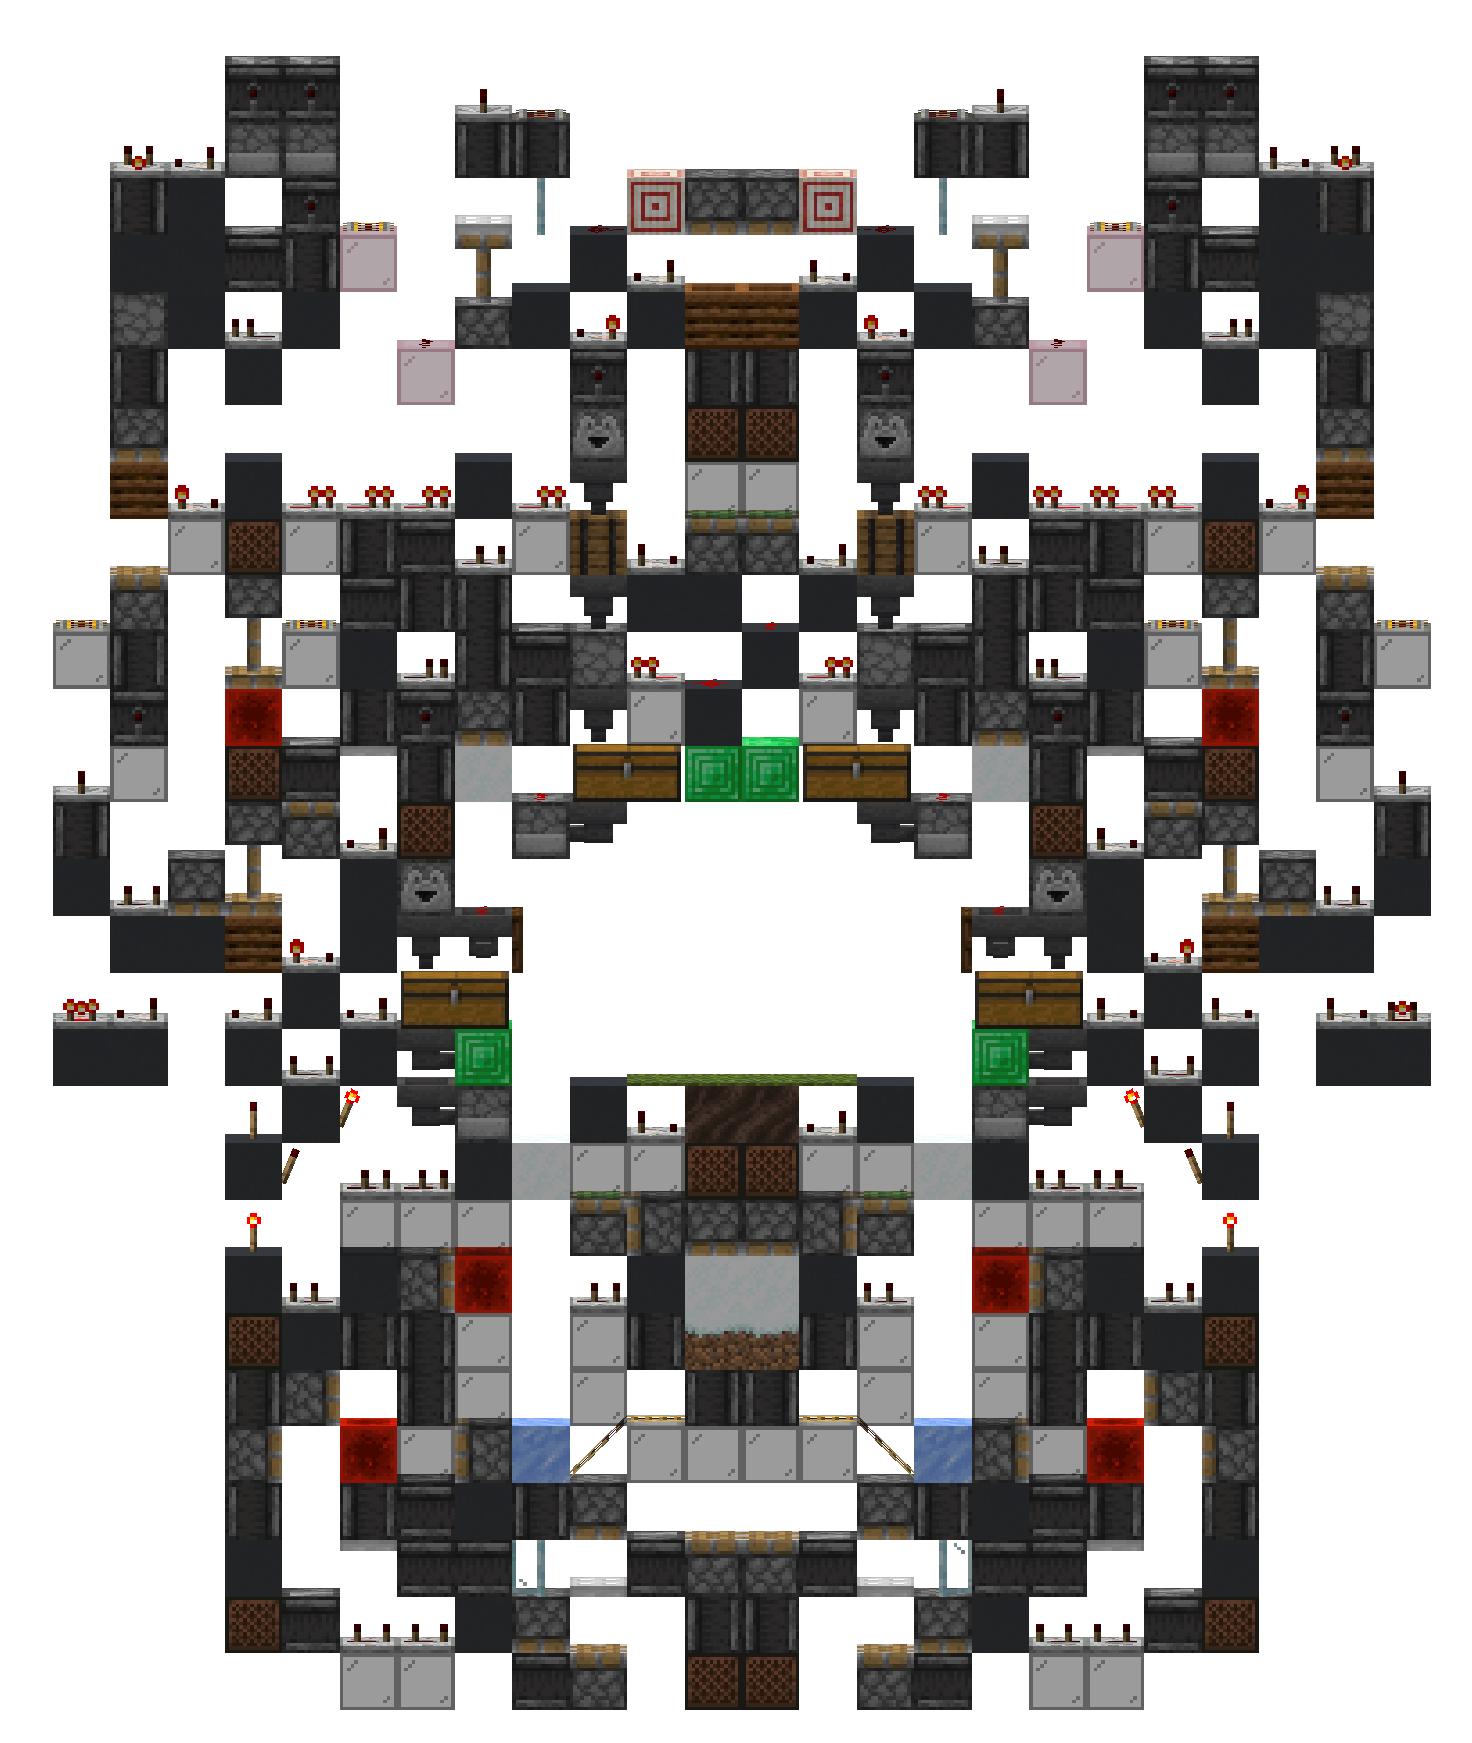
\includegraphics[width=0.48\textwidth]{slice2.png}
    \caption{\centering DH01 Quad Display Slice}
\end{figure}

% For wide tables, a single column layout is better. It can be switched
% page-by-page.
\onecolumn

\section{Device Specifications}

\begin{table}[h]
    \caption{Device Specifications}
    \begin{tabularx}{\textwidth}{l | c c c | c | X}
        \thickhline
        \textbf{Parameter} & \textbf{Min.} & \textbf{Typ.} & \textbf{Max.} &
        \textbf{Unit} & \textbf{Conditions} \\
        \hline
        Item Throughput  & 8 & - & - & gt & Normal Usage \\
        \hline
        MC Version & 1.18.2 & 1.18.2 & - & MCV & Latest version at time of writing: 1.19.3\\
        \hline
        Dimensions & & 1 x 29 x 24 & & Blocks & \\
        \thickhline
\end{tabularx}
\end{table}
\newpage
\section{Testing Data}
\begin{table}[h]
\caption{Executed Tests}
\begin{tabularx}{\textwidth}{l | X}
    \thickhline
    \textbf{Test} & \textbf{Result} \\
    \hline
    Display operation & Box displays were able to replace boxes when emptied. \\
    \hline
    Display spam & Box displays did not break with items being taken in and out of box rapidly. \\
    \thickhline
\end{tabularx}
\end{table}

\section{Download Information}
\begin{table}[h]
    \caption{Download Information}
    \begin{tabularx}{\textwidth}{l | l | l | X}
        \thickhline
        \textbf{Identifier} & \textbf{MC} & \textbf{File} & \textbf{Description} \\
        \hline
        DH01 & 1.18.2 & \href{https://github.com/Soontech-Annals/Archive/blob/8413f90a054b6c415703bae02badeba7541344f6/Archive/display-halls/DH01\%20Quad\%20Display\%20Slice\%20With\%20Reliable\%20Collection/DH01\_quad\_display\_slice.litematic?raw=1}{DH01\_quad\_display\_slice.litematic} & Litematic of slice. \\
        \hline
        \thickhline
    \end{tabularx}
\end{table}

\end{document}

